\documentclass[aspectratio=169]{beamer}
\usetheme{Madrid}
\usecolortheme{default}

\usepackage{amsmath}
\usepackage{amssymb}
\usepackage{amsthm}
\usepackage{tikz}
\usepackage{pgfplots}
\pgfplotsset{compat=1.17}

% Remove navigation symbols
\setbeamertemplate{navigation symbols}{}

\title{Intermediate Value Theorem, Sequences \& L'Hôpital's Rule}
\author{Mathematics for ML}
\date{\today}

\begin{document}

\frame{\titlepage}

\begin{frame}{Outline}
\tableofcontents
\end{frame}

\section{The Intermediate Value Theorem}

\begin{frame}{Intermediate Value Theorem: Statement}
\begin{theorem}[Intermediate Value Theorem (IVT)]
Let $f$ be a \textbf{continuous} function on the closed interval $[a, b]$.

If $k$ is any value between $f(a)$ and $f(b)$, then there exists at least one point $c \in (a, b)$ such that:
$$f(c) = k$$
\end{theorem}

\vspace{0.5cm}

\textbf{Intuitive Meaning:}
\begin{itemize}
    \item A continuous function must pass through every value between $f(a)$ and $f(b)$
    \item You cannot "jump over" values
    \item \textcolor{red}{Continuity is essential!}
\end{itemize}
\end{frame}

\begin{frame}{IVT: Visual Illustration}
\begin{center}
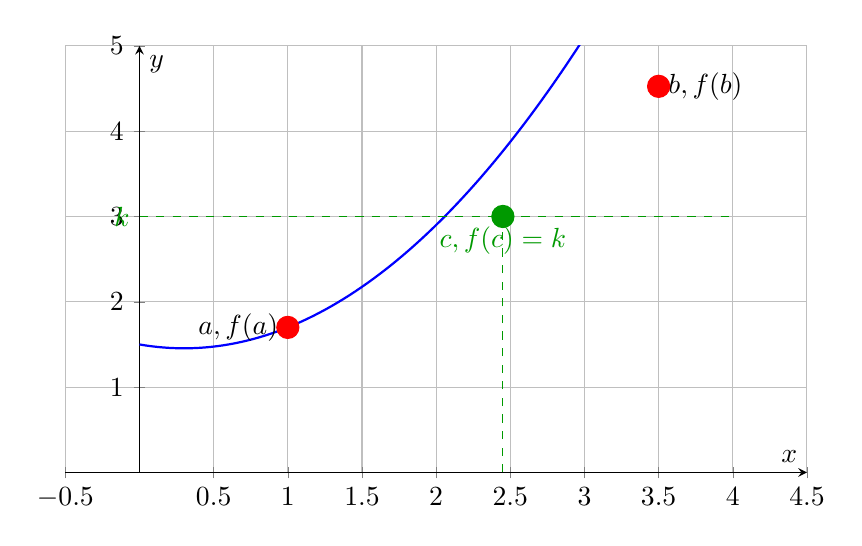
\begin{tikzpicture}
\begin{axis}[
    axis lines=middle,
    xlabel={$x$},
    ylabel={$y$},
    domain=0:4,
    samples=100,
    width=11cm,
    height=7cm,
    ymin=0, ymax=5,
    xmin=-0.5, xmax=4.5,
    grid=major
]
% Continuous function
\addplot[blue, thick] {0.5*x^2 - 0.3*x + 1.5};

% Mark endpoints
\addplot[red, only marks, mark=*, mark size=4pt] coordinates {(1, 1.7) (3.5, 4.525)};
\node[left] at (axis cs:1, 1.7) {$a, f(a)$};
\node[right] at (axis cs:3.5, 4.525) {$b, f(b)$};

% Mark intermediate value
\addplot[green!60!black, dashed] coordinates {(0, 3) (4, 3)};
\node[left, green!60!black] at (axis cs:0, 3) {$k$};

% Mark where f(c) = k
\addplot[green!60!black, only marks, mark=*, mark size=4pt] coordinates {(2.45, 3)};
\node[below, green!60!black] at (axis cs:2.45, 3) {$c, f(c)=k$};
\draw[green!60!black, dashed] (axis cs:2.45, 0) -- (axis cs:2.45, 3);
\end{axis}
\end{tikzpicture}
\end{center}

Since $f$ is continuous and $f(a) < k < f(b)$, there exists $c$ with $f(c) = k$.
\end{frame}

\begin{frame}{Why Continuity Matters}
\textbf{Without continuity, IVT fails!}

\begin{center}
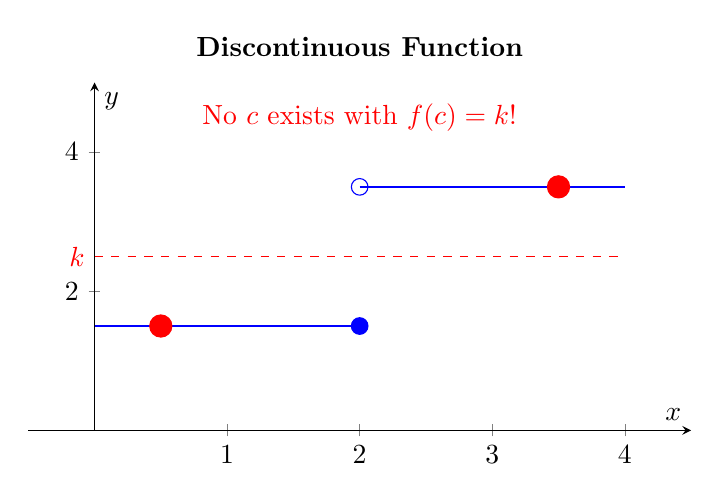
\begin{tikzpicture}
\begin{axis}[
    axis lines=middle,
    xlabel={$x$},
    ylabel={$y$},
    domain=0:4,
    samples=100,
    width=10cm,
    height=6cm,
    ymin=0, ymax=5,
    xmin=-0.5, xmax=4.5,
    title={\textbf{Discontinuous Function}}
]
% Discontinuous function
\addplot[blue, thick, domain=0:2] {1.5};
\addplot[blue, thick, domain=2:4] {3.5};

% Show the jump
\addplot[blue, only marks, mark=*, mark size=3pt] coordinates {(2, 1.5)};
\addplot[blue, only marks, mark=o, mark size=3pt] coordinates {(2, 3.5)};

% Mark endpoints
\addplot[red, only marks, mark=*, mark size=4pt] coordinates {(0.5, 1.5) (3.5, 3.5)};

% Show missing value
\addplot[red, dashed] coordinates {(0, 2.5) (4, 2.5)};
\node[left, red] at (axis cs:0, 2.5) {$k$};
\node[red] at (axis cs:2, 4.5) {No $c$ exists with $f(c) = k$!};
\end{axis}
\end{tikzpicture}
\end{center}
\end{frame}

\begin{frame}{Proof of IVT (Sketch)}
\textbf{Proof Idea:} Use the \textit{bisection method} and completeness of $\mathbb{R}$.

\vspace{0.3cm}

Without loss of generality, assume $f(a) < k < f(b)$.

\begin{enumerate}
    \item \textbf{Define sets:} 
    $$A = \{x \in [a,b] : f(x) \leq k\}$$
    $$B = \{x \in [a,b] : f(x) \geq k\}$$
    
    \item Note: $a \in A$ (since $f(a) < k$) and $b \in B$ (since $f(b) > k$)
    
    \item $A$ is non-empty and bounded above by $b$
    
    \item By completeness of $\mathbb{R}$, $c = \sup A$ exists
    
    \item By continuity: $f(c) = \lim_{x \to c} f(x)$
    
    \item Since $c = \sup A$, we can find sequences $x_n \in A$ with $x_n \to c$
    
    \item Thus $f(x_n) \leq k$ for all $n$, so $f(c) = \lim f(x_n) \leq k$
\end{enumerate}
\end{frame}

\begin{frame}{Proof of IVT (continued)}
\begin{enumerate}
    \setcounter{enumi}{6}
    \item Similarly, for any $\epsilon > 0$, since $c$ is least upper bound of $A$, there exists $y \in (c, c+\epsilon) \cap B$
    
    \item For such $y$: $f(y) \geq k$
    
    \item Taking $y \to c^+$, by continuity: $f(c) \geq k$
    
    \item Combining: $f(c) \leq k$ and $f(c) \geq k$
    
    \item Therefore: $f(c) = k$ \qed
\end{enumerate}

\vspace{0.5cm}

\textbf{Key Ideas Used:}
\begin{itemize}
    \item Completeness of real numbers (supremum exists)
    \item Definition of continuity
    \item Properties of limits
\end{itemize}
\end{frame}

\begin{frame}{Example 1: Root Finding}
\textbf{Problem:} Prove that $f(x) = x^3 - x - 1$ has a root in $[1, 2]$.

\vspace{0.3cm}

\textbf{Solution:}
\begin{enumerate}
    \item Check that $f$ is continuous (polynomial $\Rightarrow$ continuous)
    
    \item Evaluate at endpoints:
    \begin{align*}
        f(1) &= 1^3 - 1 - 1 = -1 < 0 \\
        f(2) &= 2^3 - 2 - 1 = 5 > 0
    \end{align*}
    
    \item Since $f(1) < 0 < f(2)$ and $f$ is continuous on $[1, 2]$
    
    \item By IVT: $\exists c \in (1, 2)$ such that $f(c) = 0$
\end{enumerate}

\vspace{0.3cm}

\textbf{Conclusion:} The equation $x^3 - x - 1 = 0$ has at least one solution in $(1, 2)$.
\end{frame}

\begin{frame}{Example 1: Visualization}
\begin{center}
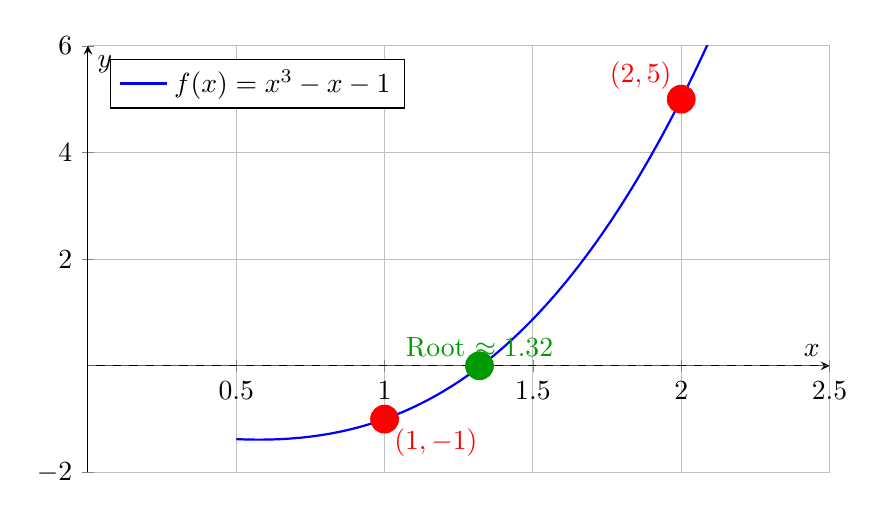
\begin{tikzpicture}
\begin{axis}[
    axis lines=middle,
    xlabel={$x$},
    ylabel={$y$},
    domain=0.5:2.5,
    samples=100,
    width=11cm,
    height=7cm,
    ymin=-2, ymax=6,
    grid=major,
    legend pos=north west
]
\addplot[blue, thick] {x^3 - x - 1};
\addlegendentry{$f(x) = x^3 - x - 1$}

% Mark endpoints
\addplot[red, only marks, mark=*, mark size=5pt] coordinates {(1, -1) (2, 5)};
\node[below right, red] at (axis cs:1, -1) {$(1, -1)$};
\node[above left, red] at (axis cs:2, 5) {$(2, 5)$};

% Show x-axis crossing
\addplot[green!60!black, dashed] coordinates {(0, 0) (2.5, 0)};

% Approximate root
\addplot[green!60!black, only marks, mark=*, mark size=5pt] coordinates {(1.32, 0)};
\node[above, green!60!black] at (axis cs:1.32, 0) {Root $\approx 1.32$};
\end{axis}
\end{tikzpicture}
\end{center}
\end{frame}

\begin{frame}{Example 2: Fixed Point Theorem}
\textbf{Problem:} Show that $g(x) = \cos(x)$ has a fixed point in $[0, \pi/2]$.

(A \textbf{fixed point} means $g(c) = c$ for some $c$)

\vspace{0.3cm}

\textbf{Solution:}
\begin{enumerate}
    \item Define $f(x) = g(x) - x = \cos(x) - x$
    
    \item $f$ is continuous on $[0, \pi/2]$ (difference of continuous functions)
    
    \item Evaluate at endpoints:
    \begin{align*}
        f(0) &= \cos(0) - 0 = 1 - 0 = 1 > 0 \\
        f(\pi/2) &= \cos(\pi/2) - \pi/2 = 0 - \pi/2 < 0
    \end{align*}
    
    \item Since $f(0) > 0 > f(\pi/2)$, by IVT: $\exists c \in (0, \pi/2)$ with $f(c) = 0$
    
    \item Thus $\cos(c) - c = 0$, i.e., $\cos(c) = c$
\end{enumerate}
\end{frame}

\section{Infinite Sequences}

\begin{frame}{Sequences: Definition}
\begin{definition}
An \textbf{infinite sequence} is a function from $\mathbb{N}$ to $\mathbb{R}$:
$$a: \mathbb{N} \to \mathbb{R}, \quad n \mapsto a_n$$
We write: $\{a_n\}_{n=1}^{\infty}$ or simply $\{a_n\}$
\end{definition}

\vspace{0.3cm}

\textbf{Examples:}
\begin{enumerate}
    \item $a_n = \frac{1}{n}$: \quad $1, \frac{1}{2}, \frac{1}{3}, \frac{1}{4}, \ldots$
    
    \item $a_n = (-1)^n$: \quad $-1, 1, -1, 1, -1, \ldots$
    
    \item $a_n = \frac{n}{n+1}$: \quad $\frac{1}{2}, \frac{2}{3}, \frac{3}{4}, \frac{4}{5}, \ldots$
    
    \item $a_n = n^2$: \quad $1, 4, 9, 16, 25, \ldots$
\end{enumerate}
\end{frame}

\begin{frame}{Convergence of Sequences}
\begin{definition}
A sequence $\{a_n\}$ \textbf{converges} to $L$ if:
$$\forall \epsilon > 0, \exists N \in \mathbb{N} \text{ such that } \forall n > N: |a_n - L| < \epsilon$$

We write: $\lim_{n \to \infty} a_n = L$ or $a_n \to L$
\end{definition}

\vspace{0.3cm}

\textbf{Intuitive Meaning:}
\begin{itemize}
    \item Terms get arbitrarily close to $L$ as $n$ increases
    \item For any tolerance $\epsilon$, eventually all terms are within $\epsilon$ of $L$
    \item The sequence "settles down" to $L$
\end{itemize}

\vspace{0.3cm}

\textbf{Divergence:} If no such $L$ exists, the sequence \textbf{diverges}.
\end{frame}

\begin{frame}{Convergence: Visual}
\begin{center}
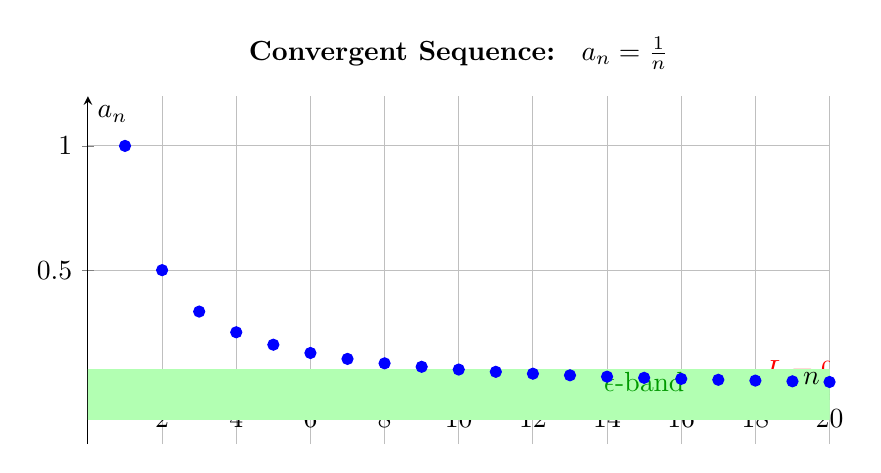
\begin{tikzpicture}
\begin{axis}[
    axis lines=middle,
    xlabel={$n$},
    ylabel={$a_n$},
    domain=1:20,
    samples at={1,2,...,20},
    width=11cm,
    height=6cm,
    ymin=-0.2, ymax=1.2,
    grid=major,
    title={\textbf{Convergent Sequence: } $a_n = \frac{1}{n}$}
]
\addplot[blue, only marks, mark=*] {1/x};

% Show limit line
\addplot[red, thick, dashed] coordinates {(0, 0) (20, 0)};
\node[red, right] at (axis cs:18, 0.1) {$L = 0$};

% Show epsilon band
\addplot[green!30, fill] coordinates {(0, -0.1) (20, -0.1) (20, 0.1) (0, 0.1)} -- cycle;
\node[green!60!black] at (axis cs:15, 0.05) {$\epsilon$-band};
\end{axis}
\end{tikzpicture}
\end{center}
\end{frame}

\begin{frame}{Important Sequence Limits}
\textbf{Common Limits:}

\begin{enumerate}
    \item $\lim_{n \to \infty} \frac{1}{n^p} = 0$ \quad for any $p > 0$
    
    \item $\lim_{n \to \infty} r^n = 0$ \quad if $|r| < 1$
    
    \item $\lim_{n \to \infty} r^n = \infty$ \quad if $r > 1$
    
    \item $\lim_{n \to \infty} r^n$ does not exist if $r \leq -1$
    
    \item $\lim_{n \to \infty} \left(1 + \frac{1}{n}\right)^n = e$
    
    \item $\lim_{n \to \infty} \frac{n}{n+1} = 1$
    
    \item $\lim_{n \to \infty} \frac{a_n}{b_n} = \frac{\lim a_n}{\lim b_n}$ \quad (if limits exist and $\lim b_n \neq 0$)
\end{enumerate}
\end{frame}

\begin{frame}{Properties of Limits}
\begin{theorem}
If $\lim_{n \to \infty} a_n = L$ and $\lim_{n \to \infty} b_n = M$, then:

\begin{enumerate}
    \item $\lim_{n \to \infty} (a_n + b_n) = L + M$
    
    \item $\lim_{n \to \infty} (c \cdot a_n) = c \cdot L$ \quad for any constant $c$
    
    \item $\lim_{n \to \infty} (a_n \cdot b_n) = L \cdot M$
    
    \item $\lim_{n \to \infty} \frac{a_n}{b_n} = \frac{L}{M}$ \quad if $M \neq 0$
    
    \item If $a_n \leq b_n$ for all $n$, then $L \leq M$
\end{enumerate}
\end{theorem}

\vspace{0.3cm}

\textbf{Squeeze Theorem:} If $a_n \leq c_n \leq b_n$ and $\lim a_n = \lim b_n = L$, then $\lim c_n = L$.
\end{frame}

\begin{frame}{Example 3: Prove Convergence}
\textbf{Problem:} Prove that $\lim_{n \to \infty} \frac{2n + 3}{n + 1} = 2$.

\vspace{0.3cm}

\textbf{Proof:}

Given $\epsilon > 0$, we need to find $N$ such that for all $n > N$:
$$\left|\frac{2n + 3}{n + 1} - 2\right| < \epsilon$$

\begin{align*}
\left|\frac{2n + 3}{n + 1} - 2\right| &= \left|\frac{2n + 3 - 2(n+1)}{n + 1}\right| \\
&= \left|\frac{2n + 3 - 2n - 2}{n + 1}\right| \\
&= \left|\frac{1}{n + 1}\right| \\
&= \frac{1}{n + 1} < \epsilon
\end{align*}

This holds when $n + 1 > \frac{1}{\epsilon}$, i.e., $n > \frac{1}{\epsilon} - 1$.

Choose $N = \lceil \frac{1}{\epsilon} \rceil$. Then for all $n > N$, we have $\left|\frac{2n+3}{n+1} - 2\right| < \epsilon$. \qed
\end{frame}

\begin{frame}{Monotone Convergence Theorem}
\begin{theorem}[Monotone Convergence Theorem]
\begin{enumerate}
    \item If $\{a_n\}$ is \textbf{increasing} and \textbf{bounded above}, then $\{a_n\}$ converges to $\sup\{a_n\}$
    
    \item If $\{a_n\}$ is \textbf{decreasing} and \textbf{bounded below}, then $\{a_n\}$ converges to $\inf\{a_n\}$
\end{enumerate}
\end{theorem}

\vspace{0.3cm}

\textbf{Proof Sketch (for increasing case):}
\begin{enumerate}
    \item Let $L = \sup\{a_n\}$ (exists by completeness)
    \item For any $\epsilon > 0$, $L - \epsilon$ is not an upper bound
    \item So $\exists N$ with $a_N > L - \epsilon$
    \item Since $\{a_n\}$ is increasing: $a_n \geq a_N > L - \epsilon$ for all $n \geq N$
    \item Also $a_n \leq L < L + \epsilon$ (since $L$ is supremum)
    \item Thus $|a_n - L| < \epsilon$ for all $n \geq N$ \qed
\end{enumerate}
\end{frame}

\section{L'Hôpital's Rule}

\begin{frame}{L'Hôpital's Rule: Statement}
\begin{theorem}[L'Hôpital's Rule]
Suppose $f$ and $g$ are differentiable near $a$ (except possibly at $a$), and $g'(x) \neq 0$ near $a$.

If $\lim_{x \to a} f(x) = \lim_{x \to a} g(x) = 0$ \quad or \quad $\lim_{x \to a} |f(x)| = \lim_{x \to a} |g(x)| = \infty$

\textbf{and} if $\lim_{x \to a} \frac{f'(x)}{g'(x)}$ exists (or is $\pm \infty$), then:
$$\lim_{x \to a} \frac{f(x)}{g(x)} = \lim_{x \to a} \frac{f'(x)}{g'(x)}$$
\end{theorem}

\vspace{0.3cm}

\textbf{Note:} This also works for:
\begin{itemize}
    \item One-sided limits ($x \to a^+$ or $x \to a^-$)
    \item Limits at infinity ($x \to \infty$ or $x \to -\infty$)
\end{itemize}
\end{frame}

\begin{frame}{Indeterminate Forms}
L'Hôpital's Rule applies to \textbf{indeterminate forms}:

\vspace{0.3cm}

\textbf{Direct Application:}
\begin{itemize}
    \item $\frac{0}{0}$ form: Both numerator and denominator approach 0
    \item $\frac{\infty}{\infty}$ form: Both approach infinity
\end{itemize}

\vspace{0.3cm}

\textbf{Can be converted:}
\begin{itemize}
    \item $0 \cdot \infty$ form: Rewrite as $\frac{0}{1/\infty}$ or $\frac{\infty}{1/0}$
    \item $\infty - \infty$ form: Combine into single fraction
    \item $0^0$, $1^{\infty}$, $\infty^0$ forms: Use logarithms
\end{itemize}

\vspace{0.3cm}

\textbf{Warning:} L'Hôpital's Rule does NOT apply if the limit is not indeterminate!
\end{frame}

\begin{frame}{Proof of L'Hôpital's Rule (0/0 case)}
\textbf{Proof for $\frac{0}{0}$ form at $x = a$:}

\begin{enumerate}
    \item Assume $f(a) = g(a) = 0$ (can extend by continuity)
    
    \item By Cauchy's Mean Value Theorem: For $x$ near $a$, $\exists c$ between $a$ and $x$ such that:
    $$\frac{f(x) - f(a)}{g(x) - g(a)} = \frac{f'(c)}{g'(c)}$$
    
    \item Since $f(a) = g(a) = 0$:
    $$\frac{f(x)}{g(x)} = \frac{f'(c)}{g'(c)}$$
    
    \item As $x \to a$, we have $c \to a$ (since $c$ is between $a$ and $x$)
    
    \item If $\lim_{x \to a} \frac{f'(x)}{g'(x)} = L$, then:
    $$\lim_{x \to a} \frac{f(x)}{g(x)} = \lim_{c \to a} \frac{f'(c)}{g'(c)} = L$$
\end{enumerate}

\qed
\end{frame}

\begin{frame}{Example 4: Basic L'Hôpital Application}
\textbf{Problem:} Evaluate $\lim_{x \to 0} \frac{\sin(x)}{x}$

\vspace{0.3cm}

\textbf{Solution:}
\begin{enumerate}
    \item Check the form: $\lim_{x \to 0} \sin(x) = 0$ and $\lim_{x \to 0} x = 0$
    
    \item This is $\frac{0}{0}$ form, so apply L'Hôpital's Rule
    
    \item Take derivatives:
    $$\lim_{x \to 0} \frac{\sin(x)}{x} = \lim_{x \to 0} \frac{(\sin x)'}{(x)'} = \lim_{x \to 0} \frac{\cos(x)}{1}$$
    
    \item Evaluate:
    $$\lim_{x \to 0} \cos(x) = \cos(0) = 1$$
\end{enumerate}

\vspace{0.3cm}

\textbf{Answer:} $\lim_{x \to 0} \frac{\sin(x)}{x} = 1$
\end{frame}

\begin{frame}{Example 5: Multiple Applications}
\textbf{Problem:} Evaluate $\lim_{x \to 0} \frac{e^x - 1 - x}{x^2}$

\vspace{0.3cm}

\textbf{Solution:}
\begin{enumerate}
    \item Check: $e^0 - 1 - 0 = 0$ and $0^2 = 0$, so this is $\frac{0}{0}$
    
    \item Apply L'Hôpital's Rule:
    $$\lim_{x \to 0} \frac{e^x - 1 - x}{x^2} = \lim_{x \to 0} \frac{e^x - 1}{2x}$$
    
    \item Still $\frac{0}{0}$! Apply again:
    $$\lim_{x \to 0} \frac{e^x - 1}{2x} = \lim_{x \to 0} \frac{e^x}{2}$$
    
    \item Evaluate:
    $$\lim_{x \to 0} \frac{e^x}{2} = \frac{e^0}{2} = \frac{1}{2}$$
\end{enumerate}

\vspace{0.3cm}

\textbf{Answer:} $\lim_{x \to 0} \frac{e^x - 1 - x}{x^2} = \frac{1}{2}$
\end{frame}

\begin{frame}{Example 6: Infinity/Infinity Form}
\textbf{Problem:} Evaluate $\lim_{x \to \infty} \frac{x^2}{e^x}$

\vspace{0.3cm}

\textbf{Solution:}
\begin{enumerate}
    \item As $x \to \infty$: $x^2 \to \infty$ and $e^x \to \infty$, so this is $\frac{\infty}{\infty}$
    
    \item Apply L'Hôpital's Rule:
    $$\lim_{x \to \infty} \frac{x^2}{e^x} = \lim_{x \to \infty} \frac{2x}{e^x}$$
    
    \item Still $\frac{\infty}{\infty}$! Apply again:
    $$\lim_{x \to \infty} \frac{2x}{e^x} = \lim_{x \to \infty} \frac{2}{e^x}$$
    
    \item Now evaluate:
    $$\lim_{x \to \infty} \frac{2}{e^x} = 0$$
\end{enumerate}

\vspace{0.3cm}

\textbf{Conclusion:} Exponentials grow faster than polynomials!
\end{frame}

\begin{frame}{Example 7: $0 \cdot \infty$ Form}
\textbf{Problem:} Evaluate $\lim_{x \to 0^+} x \ln(x)$

\vspace{0.3cm}

\textbf{Solution:}
\begin{enumerate}
    \item As $x \to 0^+$: $x \to 0$ and $\ln(x) \to -\infty$, so this is $0 \cdot \infty$
    
    \item Rewrite to get $\frac{\infty}{\infty}$ form:
    $$\lim_{x \to 0^+} x \ln(x) = \lim_{x \to 0^+} \frac{\ln(x)}{1/x}$$
    
    \item As $x \to 0^+$: numerator $\to -\infty$, denominator $\to +\infty$, so $\frac{-\infty}{\infty}$
    
    \item Apply L'Hôpital's Rule:
    $$\lim_{x \to 0^+} \frac{\ln(x)}{1/x} = \lim_{x \to 0^+} \frac{1/x}{-1/x^2} = \lim_{x \to 0^+} \frac{-x^2}{x} = \lim_{x \to 0^+} (-x) = 0$$
\end{enumerate}

\vspace{0.3cm}

\textbf{Answer:} $\lim_{x \to 0^+} x \ln(x) = 0$
\end{frame}

\begin{frame}{Example 8: $1^{\infty}$ Form}
\textbf{Problem:} Evaluate $\lim_{x \to 0^+} (1 + x)^{1/x}$

\vspace{0.3cm}

\textbf{Solution:} This is $1^{\infty}$ form. Use logarithms!

\begin{enumerate}
    \item Let $L = \lim_{x \to 0^+} (1 + x)^{1/x}$
    
    \item Take logarithm:
    $$\ln L = \lim_{x \to 0^+} \ln\left[(1+x)^{1/x}\right] = \lim_{x \to 0^+} \frac{\ln(1+x)}{x}$$
    
    \item This is $\frac{0}{0}$ form. Apply L'Hôpital:
    $$\ln L = \lim_{x \to 0^+} \frac{1/(1+x)}{1} = \lim_{x \to 0^+} \frac{1}{1+x} = 1$$
    
    \item Thus $\ln L = 1$, so:
    $$L = e^1 = e$$
\end{enumerate}

\vspace{0.3cm}

\textbf{Answer:} $\lim_{x \to 0^+} (1 + x)^{1/x} = e$ \quad (Definition of $e$!)
\end{frame}

\begin{frame}{Common Mistakes with L'Hôpital's Rule}
\textbf{Warning: Do NOT do these!}

\vspace{0.3cm}

\begin{enumerate}
    \item \textcolor{red}{$\times$} Using L'H\^opital when NOT indeterminate:
    $$\lim_{x \to 0} \frac{x + 1}{x + 2} = \frac{0 + 1}{0 + 2} = \frac{1}{2}$$
    No need for L'H\^opital! (Not $\frac{0}{0}$ or $\frac{\infty}{\infty}$)
    
    \item \textcolor{red}{$\times$} Using quotient rule instead of taking derivatives separately:
    $$\lim_{x \to 0} \frac{\sin x}{x} \neq \lim_{x \to 0} \frac{x\cos x - \sin x}{x^2}$$
    
    \item \textcolor{red}{$\times$} Forgetting to check if the derivative limit exists
    
    \item \textcolor{red}{$\times$} Applying infinitely many times without checking convergence
\end{enumerate}

\vspace{0.3cm}

\textbf{Always:} Verify the form, differentiate correctly, and check your answer!
\end{frame}

\section{Summary}

\begin{frame}{Summary: Three Key Theorems}
\begin{table}
\centering
\small
\begin{tabular}{|l|p{7cm}|}
\hline
\textbf{Theorem} & \textbf{Key Idea} \\
\hline
\hline
\textbf{IVT} & Continuous functions on $[a,b]$ take all intermediate values between $f(a)$ and $f(b)$. Used for proving existence of roots. \\
\hline
\textbf{Sequences} & Convergence means terms get arbitrarily close to limit. Monotone Convergence Theorem guarantees convergence for bounded monotone sequences. \\
\hline
\textbf{L'Hôpital} & For indeterminate forms $\frac{0}{0}$ or $\frac{\infty}{\infty}$, can evaluate limit of ratio by taking derivatives: $\lim \frac{f}{g} = \lim \frac{f'}{g'}$ \\
\hline
\end{tabular}
\end{table}

\vspace{0.5cm}

\textbf{Common Thread:} All use fundamental properties of real numbers (completeness, continuity, differentiability)
\end{frame}

\begin{frame}{Applications}
\textbf{Intermediate Value Theorem:}
\begin{itemize}
    \item Root finding algorithms (bisection method)
    \item Fixed point theorems
    \item Proving existence of solutions
\end{itemize}

\vspace{0.3cm}

\textbf{Sequences:}
\begin{itemize}
    \item Iterative algorithms (convergence analysis)
    \item Numerical methods (Newton's method, gradient descent)
    \item Series convergence (prerequisite)
\end{itemize}

\vspace{0.3cm}

\textbf{L'Hôpital's Rule:}
\begin{itemize}
    \item Computing difficult limits
    \item Taylor series analysis
    \item Asymptotic analysis
    \item Machine learning (analyzing loss function behavior)
\end{itemize}
\end{frame}

\begin{frame}{Practice Problems}
\textbf{IVT:}
\begin{enumerate}
    \item Prove $x^5 + x - 1 = 0$ has a root in $[0, 1]$
    \item Show $\tan(x) = x$ has infinitely many solutions
\end{enumerate}

\vspace{0.3cm}

\textbf{Sequences:}
\begin{enumerate}
    \item Prove $\lim_{n \to \infty} \frac{3n^2 + 2n}{n^2 + 1} = 3$
    \item Determine if $a_n = \frac{(-1)^n}{n}$ converges
\end{enumerate}

\vspace{0.3cm}

\textbf{L'Hôpital:}
\begin{enumerate}
    \item $\lim_{x \to 0} \frac{\tan x - x}{x^3}$
    \item $\lim_{x \to \infty} x^{1/x}$
    \item $\lim_{x \to 0^+} x^x$
\end{enumerate}
\end{frame}

\begin{frame}{}
\begin{center}
\Huge Thank You!

\vspace{1cm}

\Large Questions?

\vspace{1cm}

\normalsize
\textit{These three concepts are fundamental tools for analysis} \\
\textit{and will appear throughout calculus and beyond!}
\end{center}
\end{frame}

\end{document}
